%!TEX root = ../thesis.tex

\chapter{Anhang} % (fold)
\label{cha:anhang}

\section{SOCC Connector Config Ontologie} % (fold)
\label{sec:anhang_socc_connector_config_ontologie}

\lstinputlisting[language=XML,caption={}]{assets/listings/socc-config.owl}

% section socc_connector_config_ontologie (end)

\section{SIOC Services Authentication Module} % (fold)
\label{sec:anhang_sioc_services_authentication_module}

\lstinputlisting[language=XML,caption={}]{assets/listings/sioc-service-auth.owl}

% section sioc_services_authentication_module (end)

\section{Proof of Concept: Konfigurationsdaten} % (fold)
\label{sec:anhang_proof_of_concept_konfigurationsdaten}

\lstinputlisting[language={},caption={}]{assets/listings/poc_config_model.ttl}

% section proof_of_concept_konfigurationsdaten (end)

\section{OAuthTool} % (fold)
\label{sec:oauthtool}

Da während der Entwicklungsphase zum Testen immer mal wieder neue OAuth Accesstoken gebraucht werden, war es nach einer weile zu Umständlich diese sich immer per Hand zu holen. Deswegen wurde ein kleines Hilfsprogramm implementiert, dass ohne großen Aufwand Accesstoken für Facebook und Google+ holen kann. Abbildung \ref{fig:anhang_oauthtool} zeigt die Oberfläche des OAuthTools mit den Dialog für Google+.

\begin{figure}[ht]
    \centering
    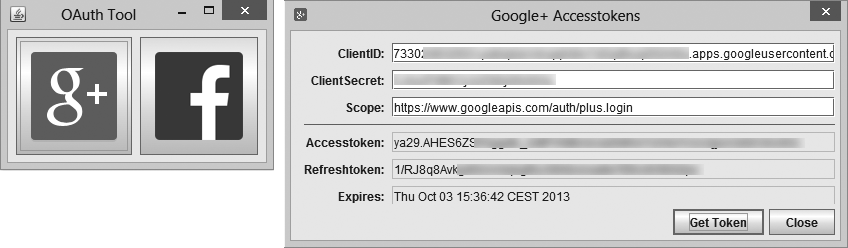
\includegraphics[
        width=\textwidth,
        keepaspectratio=true]
    {assets/images/oauthtool_windows}
    \caption{OAuthTool Fenster}
    \label{fig:anhang_oauthtool}
\end{figure}

% subsection oauthtool (end)

% section hilfsprogramme (end)

% chapter anhang (end)